\section{Auswertung}
\label{sec:Auswertung}

\subsection{Der Brechungsindex}

Zur Auswertung der aufgenommenen Messwerte werden die Brechungsindizes $n$ bei senkrechter bzw. paralleler Polarisation benötigt.
Diese können aus der Umstellung von \eqref{eq:E_rsenkrecht+snell} und \eqref{eq:E_parSnellius} gewonnen werden.
Dazu sei anzumerken, dass die gemessene Intensität proportional zum Amplitudenquadrat ist.
Es gilt also

\begin{equation}
    \frac{I_r}{I_e} \sim \frac{E_r}{E_e}^2 = E^2 \,.
    \label{eq:Intensprop}
\end{equation}


\subsubsection{Brechungsindex bei senkrechter Polarisation}
\label{subsubsec:senkPol}

Mithilfe der Definition von $E$ in \eqref{eq:Intensprop} wird \eqref{eq:E_rsenkrecht+snell} zu 

\begin{equation*}
    E_\perp = \left| \frac{\left( \sqrt{n^2 - \sin^2(\alpha)} - \cos^2(\alpha) \right)^2}{n^2 - 1} \right| \,.
\end{equation*} \\

Nach $n$ umgestellt ergibt sich dann
\begin{equation}
    n = \sqrt{1 + \frac{4 E \cos^2(\alpha)}{(E-1)^2}} \,.
    \label{eq:nsenkrecht}
\end{equation} \\

In \autoref{tab:Messung1} sind die Messwerte für die senkrechte Polarisation dargestellt. Zusätzlich dazu ist der Intensitätsquotient $E \sim \dfrac{I_r}{I_e}$ sowie 
der nach \eqref{eq:nsenkrecht} berechnete Brechungsindex aufgetragen.

\begin{table}[H]
    \centering
    \caption{Messreihe für senkrechte Polarisation.}
    \label{tab:Messung1}
    \begin{tabular}{S[table-format=2.0] S[table-format=3.0] S[table-format=1.3] S[table-format=1.3]}
      \toprule
        {Winkel $\alpha$} & {Strom $\mathbin{/} \unit{\micro\ampere}$} & {Intensitätsverhältnis $\dfrac{I_r}{I_e}$} & {$n$}\\
      \midrule
       5       &        56     &     {\dots}     &    {\dots}    \\ 
      10       &        62     &     {\dots}     &    {\dots}    \\
      15       &        67     &     {\dots}     &    {\dots}    \\
      20       &        69     &     {\dots}     &    {\dots}    \\
      25       &        71     &     {\dots}     &    {\dots}    \\
      30       &        72     &     {\dots}     &    {\dots}    \\
      35       &        77     &     {\dots}     &    {\dots}    \\
      40       &        85     &     {\dots}     &    {\dots}    \\
      45       &        84     &     {\dots}     &    {\dots}    \\
      50       &        96     &     {\dots}     &    {\dots}    \\
      55       &       100     &     {\dots}     &    {\dots}    \\
      60       &       102     &     {\dots}     &    {\dots}    \\
      65       &       108     &     {\dots}     &    {\dots}    \\
      70       &       112     &     {\dots}     &    {\dots}    \\
      75       &       139     &     {\dots}     &    {\dots}    \\
      80       &       157     &     {\dots}     &    {\dots}    \\
      85       &       160     &     {\dots}     &    {\dots}    \\
      \bottomrule
    \end{tabular}
  \end{table}

  Gemittelt ergibt sich somit ein Brechungsindex von

  \begin{equation*}
      n_\perp = ... \pm ... \,. 
  \end{equation*}

\subsubsection{Brechungsindex bei paralleler Polarisation}

Analog ergibt sich \eqref{eq:E_parSnellius} zu

\begin{equation*}
    E_\parallel = \left| \frac{n^2 \, \cos(\alpha - \sqrt{n^2 - \sin^2(\alpha)})}{n^2 \, \cos(\alpha) + \sqrt{n^2 - \sin^2(\alpha)}} \right| \,.
\end{equation*} \\

Umgestellt nach $n$ folgt

\begin{equation}
    n  = \left| \frac{1 \pm E}{cos(\alpha) (1 \pm E)} \sqrt{\frac{1}{2} 
    \left(1 + \sqrt{1 - \sin^2(2 \alpha) \frac{(1 \pm E)^2}{(1 \pm E)^2}} \right)} \right| \,,
\end{equation}

wobei $\pm E$ für $\alpha < \alpha_p$ bzw. $\alpha > \alpha_p$ fallunterschieden werden muss. \\

Wie bereits in \autoref{subsubsec:senkPol} sind in \autoref{tab:Messung2} die Messdaten, das Intensitätsverhältnis sowie der Brechungsindex für parallel polarisiertes Licht aufgetragen.

\begin{table}[H]
    \centering
    \caption{Messreihe für parallele Polarisation.}
    \label{tab:Messung2}
    \begin{tabular}{S[table-format=2.0] S[table-format=2.2] S[table-format=1.3] S[table-format=1.3]}
      \toprule
        {Winkel $\alpha$} & {Strom $\mathbin{/} \unit{\micro\ampere}$} & {Intensitätsverhältnis $\dfrac{I_r}{I_e}$} & {$n$}\\
      \midrule
       5       &       62.00    &     {\dots}    &    {\dots} \\
      10       &       62.00    &     {\dots}    &    {\dots} \\
      15       &       60.00    &     {\dots}    &    {\dots} \\
      20       &       58.00    &     {\dots}    &    {\dots} \\
      25       &       55.00    &     {\dots}    &    {\dots} \\
      30       &       50.00    &     {\dots}    &    {\dots} \\
      35       &       50.00    &     {\dots}    &    {\dots} \\
      40       &       46.00    &     {\dots}    &    {\dots} \\
      45       &       39.00    &     {\dots}    &    {\dots} \\
      50       &       34.00    &     {\dots}    &    {\dots} \\
      55       &       24.00    &     {\dots}    &    {\dots} \\
      60       &       18.00    &     {\dots}    &    {\dots} \\           
      62       &       15.00    &     {\dots}    &    {\dots} \\
      66       &        8.80    &     {\dots}    &    {\dots} \\
      70       &        3.20    &     {\dots}    &    {\dots} \\
      72       &        1.40    &     {\dots}    &    {\dots} \\
      74       &        0.85    &     {\dots}    &    {\dots} \\
      75       &        0.85    &     {\dots}    &    {\dots} \\
      78       &        5.10    &     {\dots}    &    {\dots} \\
      80       &       11.00    &     {\dots}    &    {\dots} \\  
      81       &       17.00    &     {\dots}    &    {\dots} \\
      82       &       25.00    &     {\dots}    &    {\dots} \\
      83       &       35.00    &     {\dots}    &    {\dots} \\
      84       &       50.00    &     {\dots}    &    {\dots} \\   
      85       &       52.00    &     {\dots}    &    {\dots} \\
      \bottomrule
    \end{tabular}
\end{table}

Gemittelt ergibt sich hier ein Wert von
\begin{equation*}
    n = ... \pm ...
\end{equation*}
für den Brechungsindex.

\subsection{Bestimmung des Brechungsindexes mithilfe des Brewsterwinkels}

Wie in \autoref{tab:Messung2} zu erkennen, liegt bei einem Winkel zwischen $74°$ und $75°$ ein Stromminimum vor.

Der Brewsterwinkel liegt also näherungsweise bei
\begin{equation*}
    \alpha_p = 74,5 ° \,.
\end{equation*}

Aus
\begin{equation*}
    \tan(\alpha) = n 
\end{equation*}
ergibt sich

\begin{equation*}
    n_{\alpha_p} = 3,606 \,.
\end{equation*}

In \autoref{fig:graph1} sind nun abschließend die Mess- und Theoriewerte grafisch aufgetragen. Die Theoriekurven nutzen dabei die berechneten Brechungsindizes für die senkrechte bzw. parallele Polarisation.

\begin{figure}
    \centering
    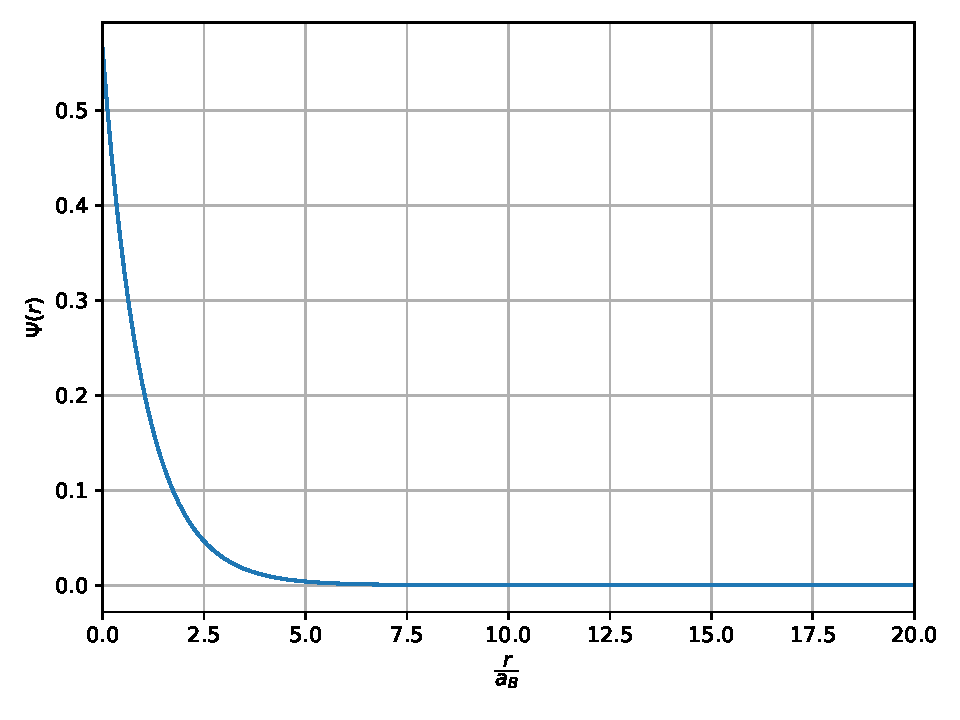
\includegraphics{build/Graph_a.pdf}
    \caption{Intensitätsverhältnis in Abhängigkeit vom Winkel $\alpha$.}
    \label{fig:graph1}
\end{figure}
